\documentclass[border=5pt]{standalone}
\usepackage{pgfplots}
\pgfplotsset{compat=1.18}
\usepackage{siunitx}
\usepackage{tikz}
\usetikzlibrary{calc}

\definecolor{trainColor}{RGB}{31,119,180}
\definecolor{valColor}{RGB}{255,127,14}

\begin{document}
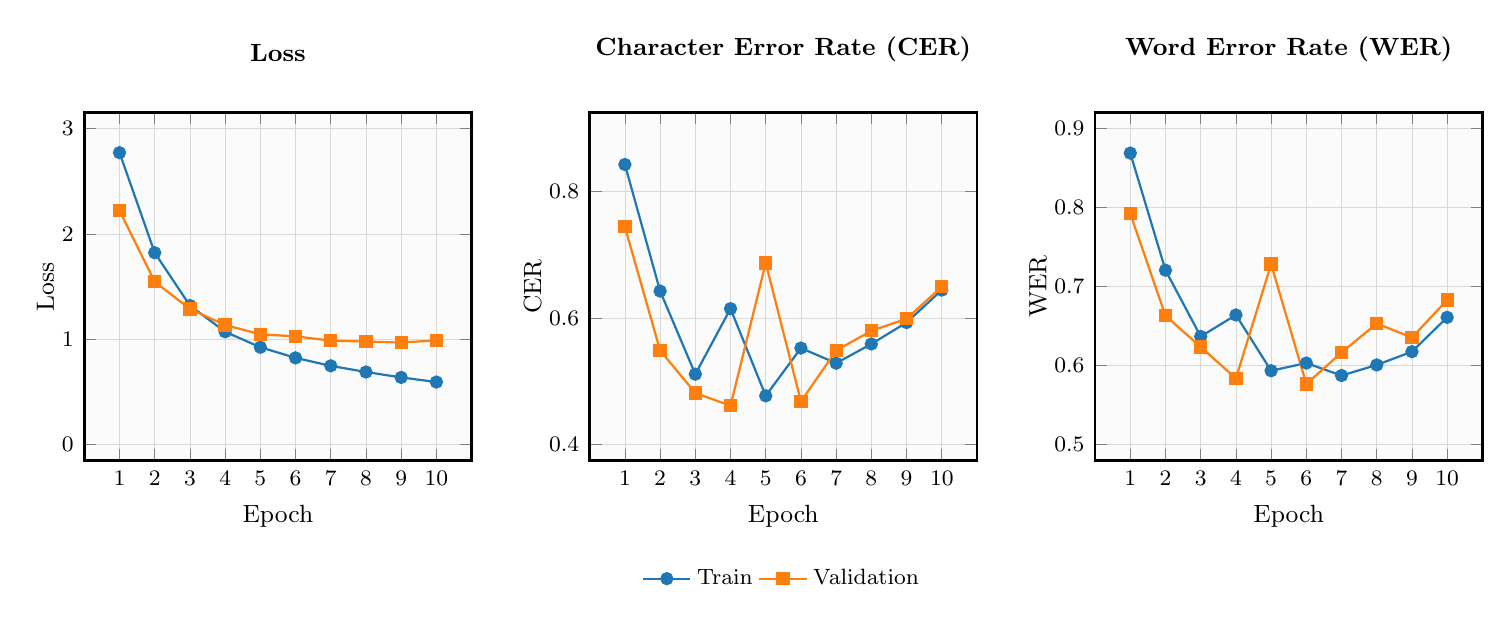
\begin{tikzpicture}[remember picture]

    % Graph 1: Loss
    \begin{axis}[
        name=plot1,
        width=6.5cm,
        height=6cm,
        xlabel={Epoch},
        ylabel={Loss},
        ylabel style={yshift=-0.15cm},
        xmin=0.5, xmax=10.5,
        ymin=0, ymax=3,
        xtick={1,2,3,4,5,6,7,8,9,10},
        grid=both,
        grid style={line width=.1pt, draw=gray!10},
        major grid style={line width=.2pt,draw=gray!30},
        title={Loss},
        axis background/.style={fill=gray!3},
        title style={yshift=3mm, font=\small\bfseries},
        label style={font=\small},
        tick label style={font=\footnotesize},
        line width=1pt,
        enlarge x limits=0.05,
        enlarge y limits=0.05,
        every axis plot/.append style={mark size=2pt},
        legend to name=commonlegend,
        legend columns=2,
        legend style={draw=none, fill=none, font=\footnotesize}
    ]
        % Train
        \addplot[color=trainColor, mark=*, thick] coordinates {
            (1, 2.7703) (2, 1.8210) (3, 1.3204) (4, 1.0714) (5, 0.9246)
            (6, 0.8239) (7, 0.7482) (8, 0.6898) (9, 0.6385) (10, 0.5945)
        };
        
        % Validation
        \addplot[color=valColor, mark=square*, thick] coordinates {
            (1, 2.2211) (2, 1.5461) (3, 1.2877) (4, 1.1357) (5, 1.0472)
            (6, 1.0280) (7, 0.9873) (8, 0.9784) (9, 0.9688) (10, 0.9901)
        };
        
        \legend{Train, Validation}
    \end{axis}
    
    % Graph 2: CER, positioned to the right of plot1
    \begin{axis}[
        name=plot2,
        at={($(plot1.east)+(1.5cm,0)$)},
        anchor=west,
        width=6.5cm,
        height=6cm,
        xlabel={Epoch},
        ylabel={CER},
        ylabel style={yshift=-0.15cm},
        xmin=0.5, xmax=10.5,
        ymin=0.4, ymax=0.9,
        xtick={1,2,3,4,5,6,7,8,9,10},
        grid=both,
        grid style={line width=.1pt, draw=gray!10},
        major grid style={line width=.2pt,draw=gray!30},
        title={Character Error Rate (CER)},
        axis background/.style={fill=gray!3},
        title style={yshift=3mm, font=\small\bfseries},
        label style={font=\small},
        tick label style={font=\footnotesize},
        line width=1pt,
        enlarge x limits=0.05,
        enlarge y limits=0.05,
        every axis plot/.append style={mark size=2pt}
    ]
        % Train
        \addplot[color=trainColor, mark=*, thick] coordinates {
            (1, 0.8430) (2, 0.6429) (3, 0.5115) (4, 0.6151) (5, 0.4773)
            (6, 0.5528) (7, 0.5289) (8, 0.5593) (9, 0.5932) (10, 0.6445)
        };
        
        % Validation
        \addplot[color=valColor, mark=square*, thick] coordinates {
            (1, 0.7445) (2, 0.5491) (3, 0.4818) (4, 0.4617) (5, 0.6874)
            (6, 0.4683) (7, 0.5489) (8, 0.5801) (9, 0.5991) (10, 0.6498)
        };
    \end{axis}
    
    % Graph 3: WER, positioned to the right of plot2
    \begin{axis}[
        name=plot3,
        at={($(plot2.east)+(1.5cm,0)$)},
        anchor=west,
        width=6.5cm,
        height=6cm,
        xlabel={Epoch},
        ylabel={WER},
        ylabel style={yshift=-0.15cm},
        xmin=0.5, xmax=10.5,
        ymin=0.5, ymax=0.9,
        xtick={1,2,3,4,5,6,7,8,9,10},
        grid=both,
        grid style={line width=.1pt, draw=gray!10},
        major grid style={line width=.2pt,draw=gray!30},
        title={Word Error Rate (WER)},
        axis background/.style={fill=gray!3},
        title style={yshift=3mm, font=\small\bfseries},
        label style={font=\small},
        tick label style={font=\footnotesize},
        line width=1pt,
        enlarge x limits=0.05,
        enlarge y limits=0.05,
        every axis plot/.append style={mark size=2pt}
    ]
        % Train
        \addplot[color=trainColor, mark=*, thick] coordinates {
            (1, 0.8688) (2, 0.7207) (3, 0.6369) (4, 0.6641) (5, 0.5936)
            (6, 0.6033) (7, 0.5875) (8, 0.6009) (9, 0.6177) (10, 0.6611)
        };
        
        % Validation
        \addplot[color=valColor, mark=square*, thick] coordinates {
            (1, 0.7922) (2, 0.6632) (3, 0.6236) (4, 0.5839) (5, 0.7284)
            (6, 0.5769) (7, 0.6165) (8, 0.6534) (9, 0.6355) (10, 0.6831)
        };
    \end{axis}

    % Positioning the common legend below all graphs
    \node at ($(plot1.south)!0.5!(plot3.south)+(0,-1.5cm)$) {\pgfplotslegendfromname{commonlegend}};
    
\end{tikzpicture}
\end{document}